

\subsection{Speech Understanding Results}
\label{section:results_speech}
We evaluate the speech understanding capabilities of our speech interface for Llama 3 on three tasks: \textbf{(1)} automatic speech recognition, \textbf{(2)} speech translation, and \textbf{(3)} spoken question answering.
We compare the performance of our speech interface for Llama 3 with three state-of-the-art models for speech understanding: Whisper \citep{radford23whisper}, SeamlessM4T \citep{barrault2023seamless}, and Gemini.\footnote{
	Due to technical limitations, we compare with the performance of Gemini on MLS reported in the original paper.
}
In all the evaluations, we used greedy search for Llama 3 token prediction.

\textbf{Speech recognition.}
We evaluate the ASR performance on the
English datasets of
Multilingual LibriSpeech (MLS; \citet{pratap2020mls}),
LibriSpeech \citep{panayotov2015librispeech},
VoxPopuli \citep{wang2021voxpopuli},
and a subset of the multilingual FLEURS dataset \citep{conneau2023fleurs}.
In evaluation, the decoding results are post-processed using the Whisper text normalizer to ensure consistency in comparing with the reported results of other models.
On all benchmarks, we measure the word error rate of our speech interface for Llama 3 on the standard test set of those benchmarks, except for Chinese, Japanese, Korean and Thai, where the character error rate is reported.



\providecommand{\bup}{($\boldsymbol\uparrow$)}
\providecommand{\bdown}{($\boldsymbol\downarrow$)}


\begin{table}[t]
	\centering
	 \resizebox{\linewidth}{!}{\begin{NiceTabular}{lcccccc}
	\CodeBefore
	\Body
	\toprule
	& \textbf{Llama 3 8B} & \textbf{Llama 3 70B} & \textbf{Whisper} & \textbf{SeamlessM4T v2} & \textbf{Gemini 1.0 Ultra} & \textbf{Gemini 1.5 Pro}\\
	\midrule
	MLS \scriptsize{(English)} & 4.9 & 4.4 & 6.2 \scriptsize{(v2)} & 6.5 & 4.4 & \textbf{4.2} \\
	LibriSpeech \scriptsize{(test-other)} & 3.4 & \textbf{3.1} & 4.9 \scriptsize{(v2)} & 6.2 & -- &  -- \\
	VoxPopuli \scriptsize{(English)}  & 6.2 & \textbf{5.7} &  7.0  \scriptsize{(v2)} & 7.0 & -- & --  \\
	FLEURS \scriptsize{(34 languages)} & 9.6 & \textbf{8.2} & 14.4 \scriptsize{(v3)}  & 11.7 & -- & -- \\
	\bottomrule
\end{NiceTabular}
}
	\caption{\textbf{Word error rate of our speech interface for Llama 3 on speech recognition tasks.} We report the performance of Whisper, SeamlessM4T, and Gemini for reference.}
	\label{table:speech_asr_results}
\end{table}


Table~\ref{table:speech_asr_results} shows the results of ASR evaluations.
It demonstrates the strong performance of Llama 3 (and multi-modal foundation models more generally) on speech recognition tasks: our model outperforms models that are tailored to speech like Whisper\footnote{On FLEURS ASR, Malayalam is not officially reported for Whisper v3, so we use the average of 33 languages.} and SeamlessM4T on all benchmarks.
On MLS English, Llama 3 performs similarly to Gemini.


\begin{table}[t]
	\centering
	\begin{NiceTabular}{lcccc}
	\CodeBefore
	\Body
	\toprule
	& \textbf{Llama 3 8B} & \textbf{Llama 3 70B} & \textbf{Whisper v2} & \textbf{SeamlessM4T v2}\\
	\midrule
	FLEURS \scriptsize{(33 lang. $\rightarrow$ English)} & 29.5 & \textbf{33.7}  & 21.9  & 28.6  \\
	Covost 2 \scriptsize{(15 lang. $\rightarrow$ English)} & 34.4 & \textbf{38.8} & 33.8  & 37.9 \\
	\bottomrule
\end{NiceTabular}

	\caption{\textbf{BLEU score of our speech interface for Llama 3 on speech translation tasks.} We report the performance of Whisper and SeamlessM4T for reference.}
	\label{table:speech_ast_results}
\end{table}


\textbf{Speech translation.}
We also evaluate our models on speech translation tasks in which the model is asked to translate non-English speech into English text.
We use the FLEURS and Covost 2 \citep{wang2021covost} datasets in these evaluations, measuring BLEU scores of the translated English.
Table~\ref{table:speech_ast_results} presents the results of these experiments.\footnote{On Covost 2, we evaluate only on 15 (out of 21) languages.} 
The performance of our models in speech translation highlights the advantages of multimodal foundation models for tasks such as speech translation. 

\begin{figure}[]
    \centering
    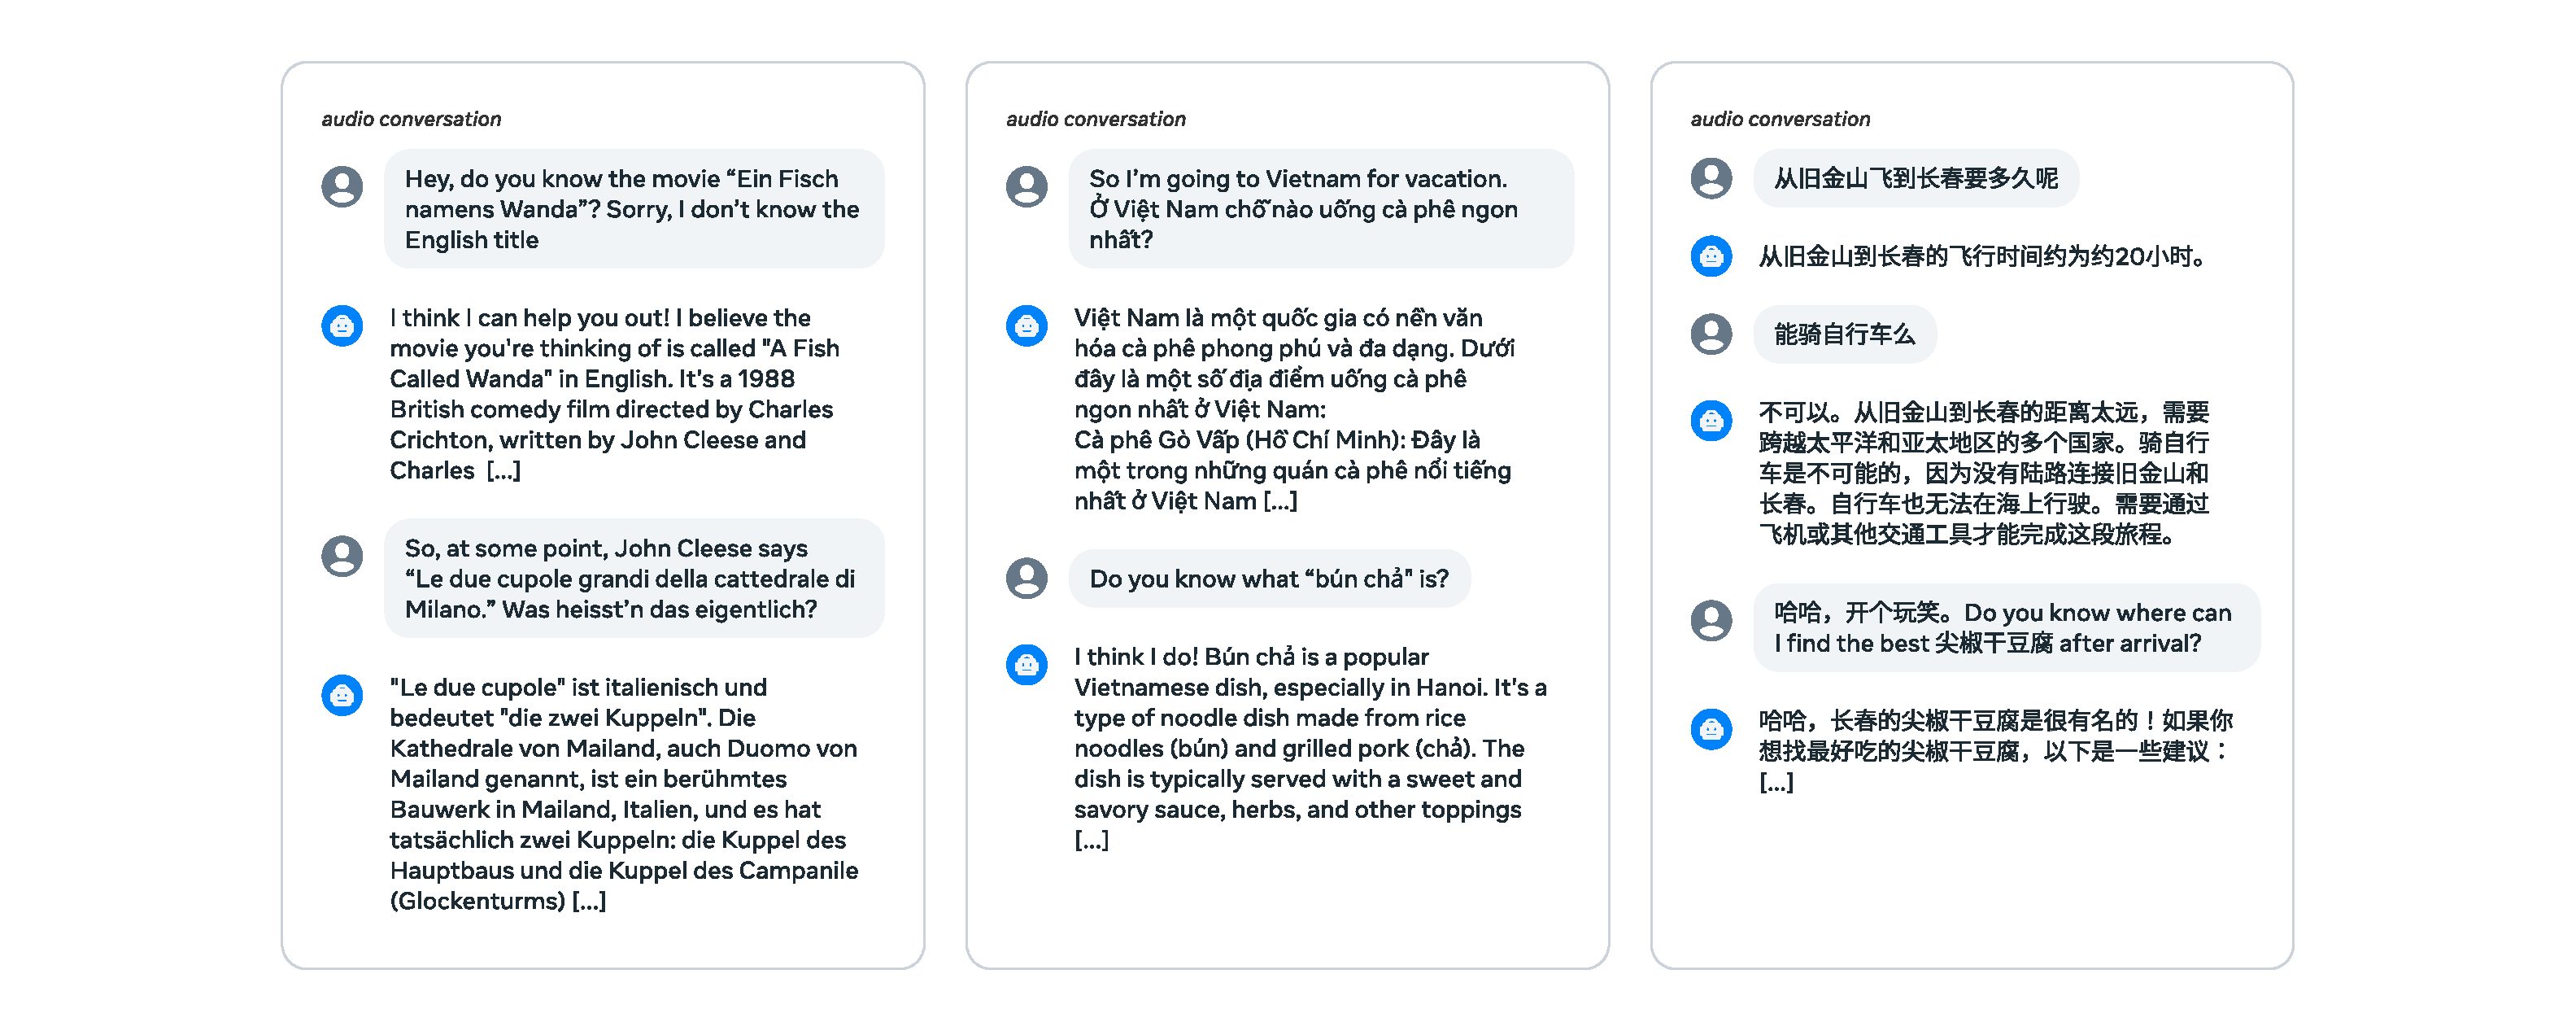
\includegraphics[trim={150px 0 150px 0},clip,width=\textwidth]{assets/llama-voice-language.pdf}
    \caption{\textbf{Transcribed dialogue examples using the speech interface for Llama 3.} The examples illustrate zero-shot multi-turn and code-switching capabilities.}
    \label{figure:speech_dialog_example}
\end{figure}

\textbf{Spoken question answering.}
The speech interface of Llama 3 demonstrates remarkable question answering capabilities. The model can effortlessly comprehend code-switched speech without any prior exposure to such data. Notably, although the model was trained only on single-turn dialogue, it is capable of engaging in extended, coherent multi-turn dialogue sessions.
Figure~\ref{figure:speech_dialog_example} presents a few examples that highlight these multilingual and multi-turn capabilities.

\begin{table}[t]
\centering
    \begin{tabular}{lcccccc}
    \toprule
     & \multicolumn{2}{c}{\textbf{Llama 3 8B}} &  \multicolumn{2}{c}{\textbf{Llama 3 70B}} & \multicolumn{2}{c}{\textbf{Gemini 1.5 Pro}} \\
    \textbf{Language} & AT \bdown & LT \bup & AT \bdown & LT  \bup & AT \bdown & LT \bup \\
    \midrule
    English & 0.84 & 15.09 & \textbf{0.68} & \textbf{15.46} & 1.44 & 13.42 \\
    Overall & 2.31 & 9.89 & \textbf{2.00} & 10.29 & 2.06 & \textbf{10.94} \\
    \bottomrule
    \end{tabular}
    \caption{\textbf{Speech toxicity of our speech interface to Llama 3 on the MuTox dataset.} AT refers to added toxicity (\%) and LT refers to lost toxicity (\%). \label{table:speech-safety-mutox}}
\end{table}

\textbf{Safety.}
We evaluate the safety of our speech model on MuTox \citep{mutox}, a multilingual audio-based dataset of 20,000 utterances for English and Spanish and 4,000 for 19 other languages, each with toxicity labels attached.
The audio is passed as input to the model and the output is evaluated for toxicity, after cleaning some special characters.
We apply the MuTox classifier~\citep{mutox} and compare the results with Gemini 1.5 Pro. We evaluate the percentage of added toxicity (AT), when the input prompt is safe and the output is toxic, and the percentage of lost toxicity (LT), when the input prompt is toxic and the answer is safe. Table~\ref{table:speech-safety-mutox} shows the results for English and an average across all 21 languages that we evaluated on.\footnote{Note that for Gemini, we encountered that a significant number of responses were empty, which could be due to safety filters on their side (though some empty responses were for non-toxic input) or to rate limits. To conduct the analysis, we assumed that all the empty responses are safe. This is the most conservative approach for results and the upper bound of what Gemini results would look like.} The percentage of added toxicity is very low: our speech models have the lowest percentage of added toxicity for English, with less than 1\%. It removes significantly more toxicity than it adds.


\subsection{Speech Generation Results}
For speech generation, we focus on evaluating the quality of token-wise input streaming models with the Llama 3 embeddings for the text normalization and prosody modeling tasks. The evaluation focuses on comparisons with models that do not take the Llama 3 embeddings as an additional input.

\textbf{Text normalization.}
To measure the effect of Llama 3 embeddings, we experimented with changing the amount of right context the model uses. We trained the model using a right context of 3 TN tokens (demarcated by unicode category). This model is compared to models that do not use the Llama 3 embeddings, using a 3-token right context or a full bi-directional context.
As expected, Table~\ref{tab:table1} shows using the full right context improves performance for the model without Llama 3 embeddings. However, the model that incorporates the Llama 3 embeddings outperforms all other models, hence enabling token-rate input/output streaming without relying on long context in the input.

\begin{wraptable}{r}{0.45\textwidth}
	\begin{NiceTabular}{lcc}
		\CodeBefore
		\Body
		\toprule
		\textbf{Model} & \textbf{Context} & \textbf{Accuracy} \\
		\midrule
		Without Llama 3 8B & 3 & 73.6\% \\
		Without Llama 3 8B & $\infty$ & 88.0\% \\
		With Llama 3 8B & 3 & \textbf{90.7\%} \\
		\bottomrule
	\end{NiceTabular}
	\caption{\textbf{Sample-wise text normalization (TN) accuracy.} We compare models with or without Llama 3 8B embeddings, and using different right-context values.\vspace{-8mm}}
	\label{tab:table1}
\end{wraptable}

\textbf{Prosody modeling.}
To evaluate the performance of the our prosody model (PM) with Llama 3 8B, we conducted two sets of human evaluation comparing models with and without Llama 3 embeddings. Raters listened to samples from different models and indicated their preferences. To generate the final speech waveform, we use an in-house transformer based acoustic model \citep{wu2021transformer} that predicts spectral features and a WaveRNN neural vocoder \citep{kalchbrenner2018efficient} to generate the final speech waveform.  %

\begin{table}[t]
	\centering
    \begin{minipage}{.48\textwidth}
      \centering
      \begin{tabular}{lcc}
		\toprule
		\textbf{Model} & \textbf{Preference} \\
		\midrule
		PM for Llama 3 8B  & \textbf{60.0\%} \\
		\small{Streaming phone-only baseline} & 40.0\% \\
		\bottomrule
      \end{tabular}
		\label{tab:tts:pm:ab_test1}
    \end{minipage}\hfill
    \begin{minipage}{.48\textwidth}
      \centering
      \begin{tabular}{lcc}
		\toprule
		\textbf{Model} & \textbf{Preference} \\
		\midrule
		PM for Llama 3 8B & \textbf{63.6\%} \\
		\small{Non-streaming phone-only baseline} & 36.4\% \\
		\bottomrule
      \end{tabular}

    \end{minipage}
    \caption{\textbf{Prosody Modeling (PM) evaluation.} \emph{Left:} Rater preferences of PM for Llama 3 8B vs. streaming phone-only baseline. \emph{Right:} Rater preferences of PM for Llama 3 8B vs. non-streaming phone-only baseline.}
    \label{tab:pm_test}

\end{table}




First, we compare directly to a streaming baseline model without Llama 3 embeddings. 
In  the second test, the Llama 3 8B PM is compared to a non-streaming baseline model without Llama 3 embeddings. 
As shown in Table~\ref{tab:pm_test}, the Llama 3 8B PM is preferred  60\% of the time compared to the streaming baseline, and 63.6\% of the time  compared to the non-streaming baseline, indicating a significant improvement in perceived quality. The key advantage of the Llama 3 8B PM is its token-wise streaming capability (Section~\ref{sec:tts:pm}), which maintains low latency during inference. This reduces the model's lookahead requirements, enabling more responsive and real-time speech synthesis compared to non-streaming baselines.
Overall, the Llama 3 8B prosody model consistently outperforms the baseline models, demonstrating its effectiveness in enhancing the naturalness and expressiveness of synthesized speech.
